\documentclass[tikz,border=12pt]{standalone}
\usepackage[T1]{fontenc}
\usepackage{mathpazo}
\usepackage{amsmath,amssymb}
\usetikzlibrary{arrows.meta, positioning, calc, decorations.pathreplacing}

\definecolor{stblue}{HTML}{7B97AD}
\definecolor{rwgold}{HTML}{B8995E}
\definecolor{sage}{HTML}{7A9A7E}
\definecolor{dkbrown}{HTML}{3D3530}
\definecolor{wmgray}{HTML}{7B7067}
\definecolor{cream}{HTML}{F9F6F0}
\definecolor{border}{HTML}{D4C9B8}
\definecolor{terracotta}{HTML}{C47A6A}

\begin{document}
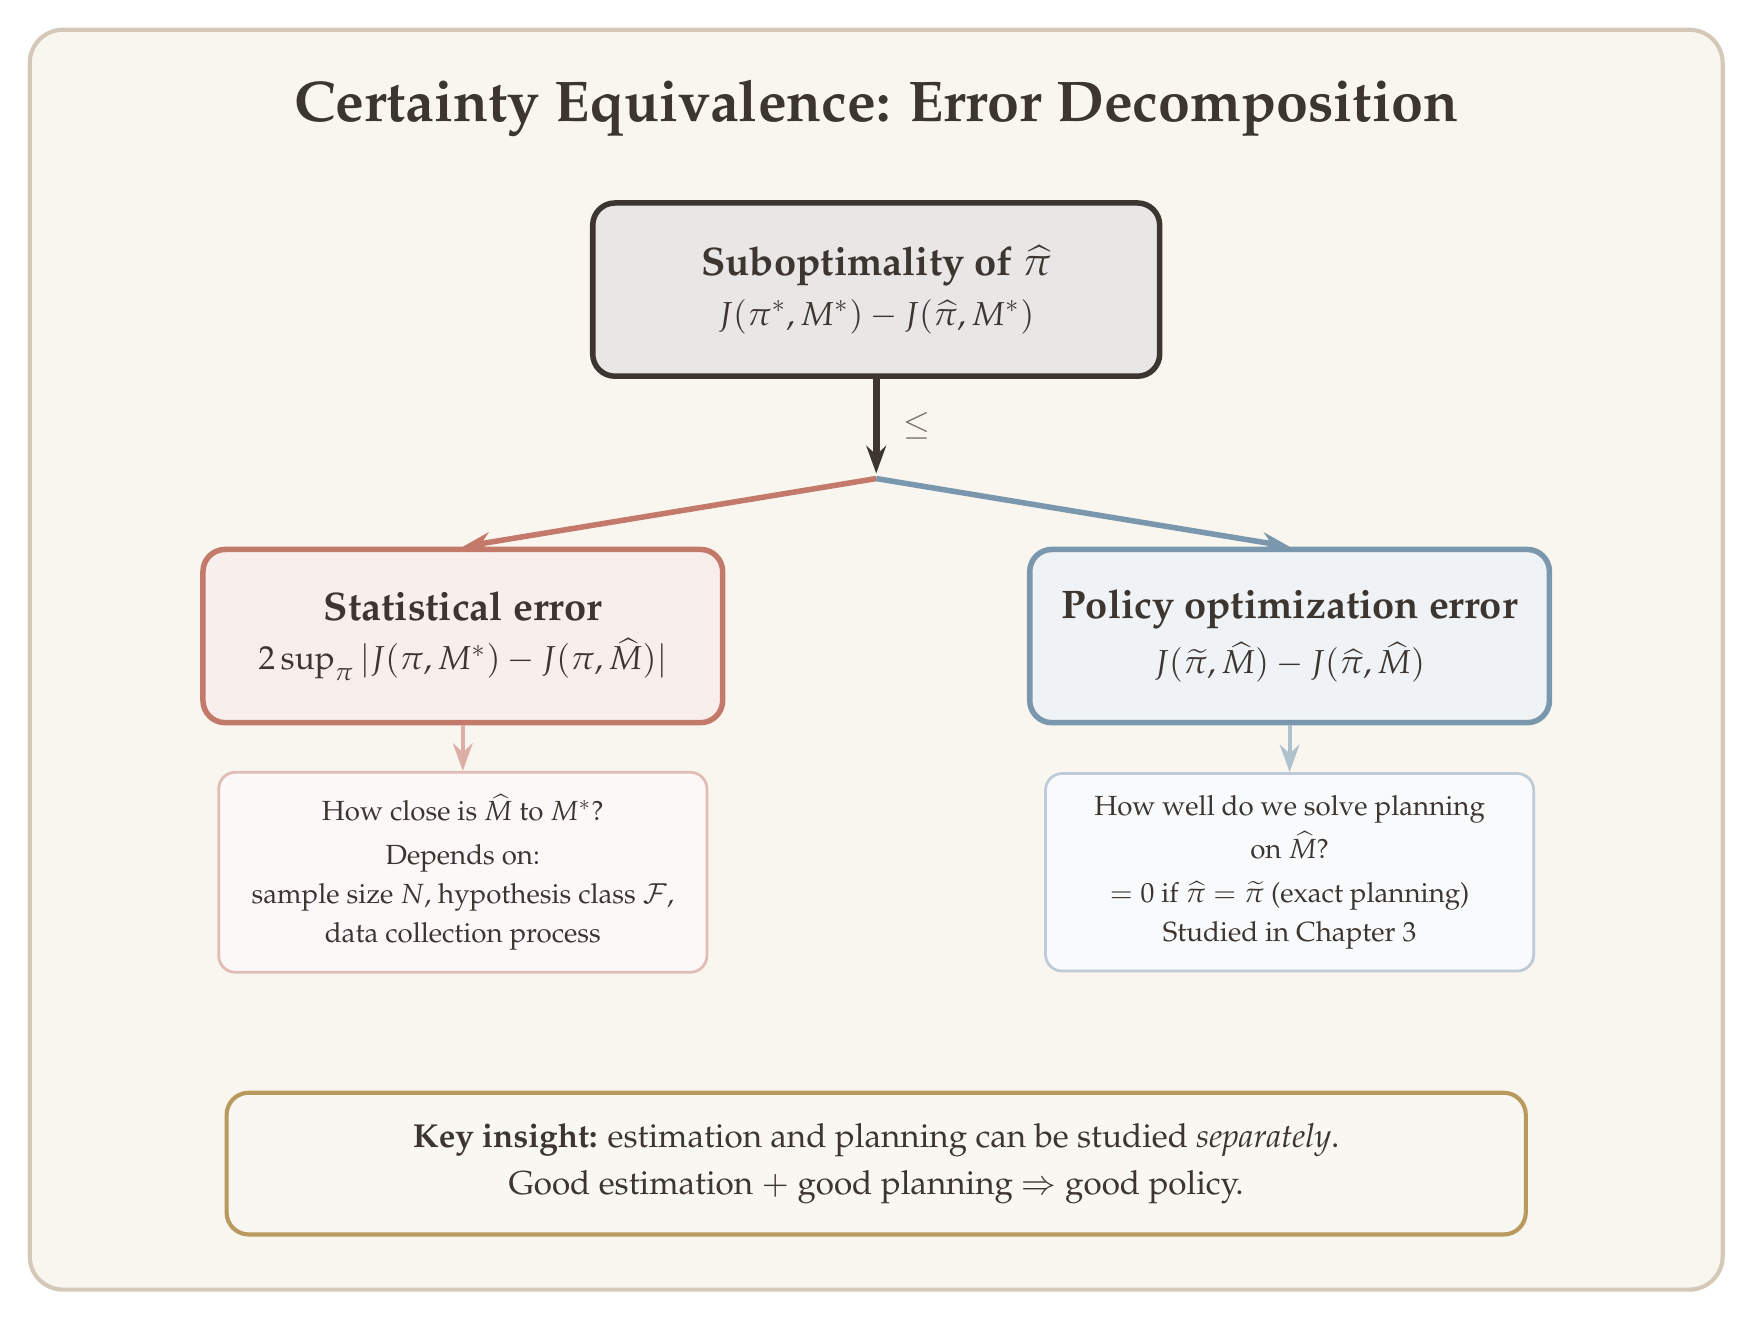
\begin{tikzpicture}[
  >={Stealth[length=3.5mm, width=2.5mm]},
  box/.style={draw=#1, line width=2pt, fill=#1!12, rounded corners=8pt,
    minimum width=58mm, minimum height=20mm, font=\large, text=dkbrown,
    align=center, inner sep=6pt},
  arr/.style={->, line width=1.8pt, dkbrown},
  lbl/.style={font=\normalsize, text=wmgray, align=center},
]

% Background
\fill[cream, rounded corners=12pt] (-1.5,-9.5) rectangle (20.0,6.5);
\draw[border, rounded corners=12pt, line width=1.5pt] (-1.5,-9.5) rectangle (20.0,6.5);

% Title
\node[font=\huge\bfseries, text=dkbrown] at (9.25,5.5)
  {Certainty Equivalence: Error Decomposition};

% === Top: Total suboptimality ===
\node[box=dkbrown, minimum width=72mm, minimum height=22mm] (total) at (9.25,3.2)
  {\textbf{\Large Suboptimality of $\widehat{\pi}$}\\[4pt]
   \large $J(\pi^*, M^*) - J(\widehat{\pi}, M^*)$};

% === Split arrow ===
\draw[arr, line width=2.5pt] (total.south) -- ++(0,-1.2)
  node[midway, right=5pt, font=\large\itshape, text=wmgray] {$\leq$};

% Branch point
\coordinate (branch) at (9.25,0.8);

% === Left: Statistical error ===
\node[box=terracotta, minimum width=66mm, minimum height=22mm] (stat) at (4.0,-1.2)
  {\textbf{\Large Statistical error}\\[4pt]
   \large $2\sup_\pi |J(\pi, M^*) - J(\pi, \widehat{M})|$};

\draw[arr, terracotta, line width=2pt] (branch) -- (stat.north);

% === Right: Policy optimization error ===
\node[box=stblue, minimum width=66mm, minimum height=22mm] (opt) at (14.5,-1.2)
  {\textbf{\Large Policy optimization error}\\[4pt]
   \large $J(\widetilde{\pi}, \widehat{M}) - J(\widehat{\pi}, \widehat{M})$};

\draw[arr, stblue, line width=2pt] (branch) -- (opt.north);

% === Below stat: what controls it ===
\node[draw=terracotta!50, line width=1pt, fill=terracotta!5,
  rounded corners=6pt, font=\normalsize, text=dkbrown, align=center,
  minimum width=62mm, inner sep=8pt] (stat_detail) at (4.0,-4.2)
  {How close is $\widehat{M}$ to $M^*$?\\[4pt]
   Depends on:\\[2pt]
   sample size $N$, hypothesis class $\mathcal{F}$,\\[2pt]
   data collection process};

\draw[arr, terracotta!60, line width=1.4pt] (stat.south) -- (stat_detail.north);

% === Below opt: what controls it ===
\node[draw=stblue!50, line width=1pt, fill=stblue!5,
  rounded corners=6pt, font=\normalsize, text=dkbrown, align=center,
  minimum width=62mm, inner sep=8pt] (opt_detail) at (14.5,-4.2)
  {How well do we solve planning\\[2pt]
   on $\widehat{M}$?\\[4pt]
   $= 0$ if $\widehat{\pi} = \widetilde{\pi}$ (exact planning)\\[2pt]
   Studied in Chapter~3};

\draw[arr, stblue!60, line width=1.4pt] (opt.south) -- (opt_detail.north);

% === Bottom: key insight ===
\draw[rwgold, line width=1.5pt, rounded corners=8pt, fill=rwgold!8]
  (1.0,-8.8) rectangle (17.5,-7.0);
\node[font=\large, text=dkbrown, align=center] at (9.25,-7.9)
  {\textbf{Key insight:} estimation and planning can be studied \emph{separately}.\\[3pt]
   Good estimation $+$ good planning $\Rightarrow$ good policy.};

\end{tikzpicture}
\end{document}
